\documentclass[1p]{elsarticle_modified}
%\bibliographystyle{elsarticle-num}

%\usepackage[colorlinks]{hyperref}
%\usepackage{abbrmath_seonhwa} %\Abb, \Ascr, \Acal ,\Abf, \Afrak
\usepackage{amsfonts}
\usepackage{amssymb}
\usepackage{amsmath}
\usepackage{amsthm}
\usepackage{scalefnt}
\usepackage{amsbsy}
\usepackage{kotex}
\usepackage{caption}
\usepackage{subfig}
\usepackage{color}
\usepackage{graphicx}
\usepackage{xcolor} %% white, black, red, green, blue, cyan, magenta, yellow
\usepackage{float}
\usepackage{setspace}
\usepackage{hyperref}

\usepackage{tikz}
\usetikzlibrary{arrows}

\usepackage{multirow}
\usepackage{array} % fixed length table
\usepackage{hhline}

%%%%%%%%%%%%%%%%%%%%%
\makeatletter
\renewcommand*\env@matrix[1][\arraystretch]{%
	\edef\arraystretch{#1}%
	\hskip -\arraycolsep
	\let\@ifnextchar\new@ifnextchar
	\array{*\c@MaxMatrixCols c}}
\makeatother %https://tex.stackexchange.com/questions/14071/how-can-i-increase-the-line-spacing-in-a-matrix
%%%%%%%%%%%%%%%

\usepackage[normalem]{ulem}

\newcommand{\msout}[1]{\ifmmode\text{\sout{\ensuremath{#1}}}\else\sout{#1}\fi}
%SOURCE: \msout is \stkout macro in https://tex.stackexchange.com/questions/20609/strikeout-in-math-mode

\newcommand{\cancel}[1]{
	\ifmmode
	{\color{red}\msout{#1}}
	\else
	{\color{red}\sout{#1}}
	\fi
}

\newcommand{\add}[1]{
	{\color{blue}\uwave{#1}}
}

\newcommand{\replace}[2]{
	\ifmmode
	{\color{red}\msout{#1}}{\color{blue}\uwave{#2}}
	\else
	{\color{red}\sout{#1}}{\color{blue}\uwave{#2}}
	\fi
}

\newcommand{\Sol}{\mathcal{S}} %segment
\newcommand{\D}{D} %diagram
\newcommand{\A}{\mathcal{A}} %arc


%%%%%%%%%%%%%%%%%%%%%%%%%%%%%5 test

\def\sl{\operatorname{\textup{SL}}(2,\Cbb)}
\def\psl{\operatorname{\textup{PSL}}(2,\Cbb)}
\def\quan{\mkern 1mu \triangleright \mkern 1mu}

\theoremstyle{definition}
\newtheorem{thm}{Theorem}[section]
\newtheorem{prop}[thm]{Proposition}
\newtheorem{lem}[thm]{Lemma}
\newtheorem{ques}[thm]{Question}
\newtheorem{cor}[thm]{Corollary}
\newtheorem{defn}[thm]{Definition}
\newtheorem{exam}[thm]{Example}
\newtheorem{rmk}[thm]{Remark}
\newtheorem{alg}[thm]{Algorithm}

\newcommand{\I}{\sqrt{-1}}
\begin{document}

%\begin{frontmatter}
%
%\title{Boundary parabolic representations of knots up to 8 crossings}
%
%%% Group authors per affiliation:
%\author{Yunhi Cho} 
%\address{Department of Mathematics, University of Seoul, Seoul, Korea}
%\ead{yhcho@uos.ac.kr}
%
%
%\author{Seonhwa Kim} %\fnref{s_kim}}
%\address{Center for Geometry and Physics, Institute for Basic Science, Pohang, 37673, Korea}
%\ead{ryeona17@ibs.re.kr}
%
%\author{Hyuk Kim}
%\address{Department of Mathematical Sciences, Seoul National University, Seoul 08826, Korea}
%\ead{hyukkim@snu.ac.kr}
%
%\author{Seokbeom Yoon}
%\address{Department of Mathematical Sciences, Seoul National University, Seoul, 08826,  Korea}
%\ead{sbyoon15@snu.ac.kr}
%
%\begin{abstract}
%We find all boundary parabolic representation of knots up to 8 crossings.
%
%\end{abstract}
%\begin{keyword}
%    \MSC[2010] 57M25 
%\end{keyword}
%
%\end{frontmatter}

%\linenumbers
%\tableofcontents
%
\newcommand\colored[1]{\textcolor{white}{\rule[-0.35ex]{0.8em}{1.4ex}}\kern-0.8em\color{red} #1}%
%\newcommand\colored[1]{\textcolor{white}{ #1}\kern-2.17ex	\textcolor{white}{ #1}\kern-1.81ex	\textcolor{white}{ #1}\kern-2.15ex\color{red}#1	}

{\Large $\underline{12a_{1263}~(K12a_{1263})}$}

\setlength{\tabcolsep}{10pt}
\renewcommand{\arraystretch}{1.6}
\vspace{1cm}\begin{tabular}{m{100pt}>{\centering\arraybackslash}m{274pt}}
\multirow{5}{120pt}{
	\centering
	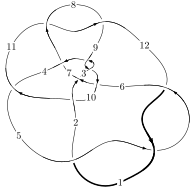
\includegraphics[width=112pt]{../../../GIT/diagram.site/Diagrams/png/2064_12a_1263.png}\\
\ \ \ A knot diagram\footnotemark}&
\allowdisplaybreaks
\textbf{Linearized knot diagam} \\
\cline{2-2}
 &
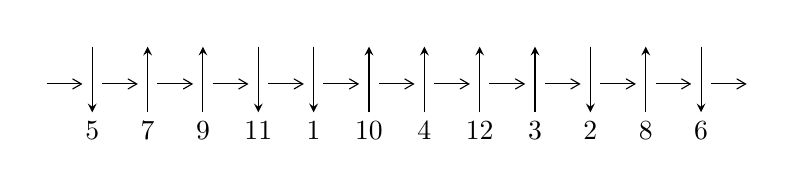
\begin{tikzpicture}[x=20pt, y=17pt]
	% nodes
	\node (C0) at (0, 0) {};
	\node (C1) at (1, 0) {};
	\node (C1U) at (1, +1) {};
	\node (C1D) at (1, -1) {5};

	\node (C2) at (2, 0) {};
	\node (C2U) at (2, +1) {};
	\node (C2D) at (2, -1) {7};

	\node (C3) at (3, 0) {};
	\node (C3U) at (3, +1) {};
	\node (C3D) at (3, -1) {9};

	\node (C4) at (4, 0) {};
	\node (C4U) at (4, +1) {};
	\node (C4D) at (4, -1) {11};

	\node (C5) at (5, 0) {};
	\node (C5U) at (5, +1) {};
	\node (C5D) at (5, -1) {1};

	\node (C6) at (6, 0) {};
	\node (C6U) at (6, +1) {};
	\node (C6D) at (6, -1) {10};

	\node (C7) at (7, 0) {};
	\node (C7U) at (7, +1) {};
	\node (C7D) at (7, -1) {4};

	\node (C8) at (8, 0) {};
	\node (C8U) at (8, +1) {};
	\node (C8D) at (8, -1) {12};

	\node (C9) at (9, 0) {};
	\node (C9U) at (9, +1) {};
	\node (C9D) at (9, -1) {3};

	\node (C10) at (10, 0) {};
	\node (C10U) at (10, +1) {};
	\node (C10D) at (10, -1) {2};

	\node (C11) at (11, 0) {};
	\node (C11U) at (11, +1) {};
	\node (C11D) at (11, -1) {8};

	\node (C12) at (12, 0) {};
	\node (C12U) at (12, +1) {};
	\node (C12D) at (12, -1) {6};
	\node (C13) at (13, 0) {};

	% arrows
	\draw[->,>={angle 60}]
	(C0) edge (C1) (C1) edge (C2) (C2) edge (C3) (C3) edge (C4) (C4) edge (C5) (C5) edge (C6) (C6) edge (C7) (C7) edge (C8) (C8) edge (C9) (C9) edge (C10) (C10) edge (C11) (C11) edge (C12) (C12) edge (C13) ;	\draw[->,>=stealth]
	(C1U) edge (C1D) (C2D) edge (C2U) (C3D) edge (C3U) (C4U) edge (C4D) (C5U) edge (C5D) (C6D) edge (C6U) (C7D) edge (C7U) (C8D) edge (C8U) (C9D) edge (C9U) (C10U) edge (C10D) (C11D) edge (C11U) (C12U) edge (C12D) ;
	\end{tikzpicture} \\
\hhline{~~} \\& 
\textbf{Solving Sequence} \\ \cline{2-2} 
 &
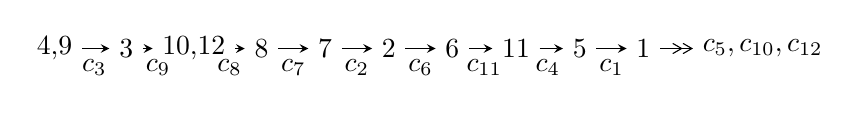
\begin{tikzpicture}[x=23pt, y=7pt]
	% node
	\node (A0) at (-1/8, 0) {4,9};
	\node (A1) at (1, 0) {3};
	\node (A2) at (33/16, 0) {10,12};
	\node (A3) at (25/8, 0) {8};
	\node (A4) at (33/8, 0) {7};
	\node (A5) at (41/8, 0) {2};
	\node (A6) at (49/8, 0) {6};
	\node (A7) at (57/8, 0) {11};
	\node (A8) at (65/8, 0) {5};
	\node (A9) at (73/8, 0) {1};
	\node (C1) at (1/2, -1) {$c_{3}$};
	\node (C2) at (3/2, -1) {$c_{9}$};
	\node (C3) at (21/8, -1) {$c_{8}$};
	\node (C4) at (29/8, -1) {$c_{7}$};
	\node (C5) at (37/8, -1) {$c_{2}$};
	\node (C6) at (45/8, -1) {$c_{6}$};
	\node (C7) at (53/8, -1) {$c_{11}$};
	\node (C8) at (61/8, -1) {$c_{4}$};
	\node (C9) at (69/8, -1) {$c_{1}$};
	\node (A10) at (11, 0) {$c_{5},c_{10},c_{12}$};

	% edge
	\draw[->,>=stealth]	
	(A0) edge (A1) (A1) edge (A2) (A2) edge (A3) (A3) edge (A4) (A4) edge (A5) (A5) edge (A6) (A6) edge (A7) (A7) edge (A8) (A8) edge (A9) ;
	\draw[->>,>={angle 60}]	
	(A9) edge (A10);
\end{tikzpicture} \\ 

\end{tabular} \\

\footnotetext{
The image of knot diagram is generated by the software ``\textbf{Draw programme}" developed by Andrew Bartholomew(\url{http://www.layer8.co.uk/maths/draw/index.htm\#Running-draw}), where we modified some parts for our purpose(\url{https://github.com/CATsTAILs/LinksPainter}).
}\phantom \\ \newline 
\centering \textbf{Ideals for irreducible components\footnotemark of $X_{\text{par}}$} 
 
\begin{align*}
I^u_{1}&=\langle 
2.24929\times10^{783} u^{139}-7.32075\times10^{782} u^{138}+\cdots+1.05867\times10^{784} b-2.31034\times10^{788},\\
\phantom{I^u_{1}}&\phantom{= \langle  }5.71289\times10^{786} u^{139}+4.97855\times10^{788} u^{138}+\cdots+1.01943\times10^{789} a-5.83232\times10^{793},\\
\phantom{I^u_{1}}&\phantom{= \langle  }u^{140}- u^{139}+\cdots+332003 u-96293\rangle \\
I^u_{2}&=\langle 
8.39783\times10^{34} u^{34}-2.36613\times10^{35} u^{33}+\cdots+6.02662\times10^{35} b-5.43593\times10^{34},\\
\phantom{I^u_{2}}&\phantom{= \langle  }8.27029\times10^{35} u^{34}-1.98216\times10^{36} u^{33}+\cdots+6.02662\times10^{35} a+1.44049\times10^{36},\;u^{35}-2 u^{34}+\cdots+2 u+1\rangle \\
\\
\end{align*}
\raggedright * 2 irreducible components of $\dim_{\mathbb{C}}=0$, with total 175 representations.\\
\footnotetext{All coefficients of polynomials are rational numbers. But the coefficients are sometimes approximated in decimal forms when there is not enough margin.}
\newpage
\renewcommand{\arraystretch}{1}
\centering \section*{I. $I^u_{1}= \langle 2.25\times10^{783} u^{139}-7.32\times10^{782} u^{138}+\cdots+1.06\times10^{784} b-2.31\times10^{788},\;5.71\times10^{786} u^{139}+4.98\times10^{788} u^{138}+\cdots+1.02\times10^{789} a-5.83\times10^{793},\;u^{140}- u^{139}+\cdots+332003 u-96293 \rangle$}
\flushleft \textbf{(i) Arc colorings}\\
\begin{tabular}{m{7pt} m{180pt} m{7pt} m{180pt} }
\flushright $a_{4}=$&$\begin{pmatrix}1\\0\end{pmatrix}$ \\
\flushright $a_{9}=$&$\begin{pmatrix}0\\u\end{pmatrix}$ \\
\flushright $a_{3}=$&$\begin{pmatrix}1\\u^2\end{pmatrix}$ \\
\flushright $a_{10}=$&$\begin{pmatrix}u\\u^3+u\end{pmatrix}$ \\
\flushright $a_{12}=$&$\begin{pmatrix}-0.00560401 u^{139}-0.488367 u^{138}+\cdots-203653. u+57211.7\\-0.212463 u^{139}+0.0691502 u^{138}+\cdots-49005.2 u+21823.0\end{pmatrix}$ \\
\flushright $a_{8}=$&$\begin{pmatrix}0.628246 u^{139}-0.450621 u^{138}+\cdots+38726.8 u-29886.8\\-0.132909 u^{139}+0.180065 u^{138}+\cdots+23446.4 u-1954.86\end{pmatrix}$ \\
\flushright $a_{7}=$&$\begin{pmatrix}0.761156 u^{139}-0.630686 u^{138}+\cdots+15280.4 u-27932.0\\-0.132909 u^{139}+0.180065 u^{138}+\cdots+23446.4 u-1954.86\end{pmatrix}$ \\
\flushright $a_{2}=$&$\begin{pmatrix}-1.68612 u^{139}+2.42121 u^{138}+\cdots+411384. u-56520.7\\-0.223495 u^{139}+0.394283 u^{138}+\cdots+73568.9 u-13608.8\end{pmatrix}$ \\
\flushright $a_{6}=$&$\begin{pmatrix}0.571880 u^{139}-0.475318 u^{138}+\cdots+10925.2 u-20445.9\\-0.166471 u^{139}+0.184555 u^{138}+\cdots+12122.7 u+2266.14\end{pmatrix}$ \\
\flushright $a_{11}=$&$\begin{pmatrix}1.28707 u^{139}-2.82130 u^{138}+\cdots-712550. u+154932.\\0.294514 u^{139}-0.651470 u^{138}+\cdots-168867. u+38137.4\end{pmatrix}$ \\
\flushright $a_{5}=$&$\begin{pmatrix}1.17734 u^{139}-0.393159 u^{138}+\cdots+290444. u-116963.\\-0.197733 u^{139}+0.442368 u^{138}+\cdots+127471. u-28333.1\end{pmatrix}$ \\
\flushright $a_{1}=$&$\begin{pmatrix}0.618210 u^{139}-2.20677 u^{138}+\cdots-703965. u+174816.\\0.0940340 u^{139}-0.645728 u^{138}+\cdots-253249. u+68008.6\end{pmatrix}$\\&\end{tabular}
\flushleft \textbf{(ii) Obstruction class $= -1$}\\~\\
\flushleft \textbf{(iii) Cusp Shapes $= -2.55798 u^{139}+3.84011 u^{138}+\cdots+744153. u-121938.$}\\~\\
\newpage\renewcommand{\arraystretch}{1}
\flushleft \textbf{(iv) u-Polynomials at the component}\newline \\
\begin{tabular}{m{50pt}|m{274pt}}
Crossings & \hspace{64pt}u-Polynomials at each crossing \\
\hline $$\begin{aligned}c_{1},c_{5},c_{12}\end{aligned}$$&$\begin{aligned}
&u^{140}+u^{139}+\cdots+111 u-19
\end{aligned}$\\
\hline $$\begin{aligned}c_{2}\end{aligned}$$&$\begin{aligned}
&u^{140}+u^{139}+\cdots-47 u^2+1
\end{aligned}$\\
\hline $$\begin{aligned}c_{3},c_{9}\end{aligned}$$&$\begin{aligned}
&u^{140}- u^{139}+\cdots+332003 u-96293
\end{aligned}$\\
\hline $$\begin{aligned}c_{4}\end{aligned}$$&$\begin{aligned}
&u^{140}- u^{139}+\cdots+119685000 u-24250000
\end{aligned}$\\
\hline $$\begin{aligned}c_{6}\end{aligned}$$&$\begin{aligned}
&u^{140}-7 u^{139}+\cdots-1123 u-3431
\end{aligned}$\\
\hline $$\begin{aligned}c_{7}\end{aligned}$$&$\begin{aligned}
&u^{140}-2 u^{139}+\cdots-1204155 u+99181
\end{aligned}$\\
\hline $$\begin{aligned}c_{8},c_{11}\end{aligned}$$&$\begin{aligned}
&u^{140}-40 u^{138}+\cdots-17417 u+6031
\end{aligned}$\\
\hline $$\begin{aligned}c_{10}\end{aligned}$$&$\begin{aligned}
&u^{140}+3 u^{139}+\cdots+206177531 u-17678239
\end{aligned}$\\
\hline
\end{tabular}\\~\\
\newpage\renewcommand{\arraystretch}{1}
\flushleft \textbf{(v) Riley Polynomials at the component}\newline \\
\begin{tabular}{m{50pt}|m{274pt}}
Crossings & \hspace{64pt}Riley Polynomials at each crossing \\
\hline $$\begin{aligned}c_{1},c_{5},c_{12}\end{aligned}$$&$\begin{aligned}
&y^{140}+141 y^{139}+\cdots-5101 y+361
\end{aligned}$\\
\hline $$\begin{aligned}c_{2}\end{aligned}$$&$\begin{aligned}
&y^{140}+3 y^{139}+\cdots-94 y+1
\end{aligned}$\\
\hline $$\begin{aligned}c_{3},c_{9}\end{aligned}$$&$\begin{aligned}
&y^{140}+87 y^{139}+\cdots+397864600249 y+9272341849
\end{aligned}$\\
\hline $$\begin{aligned}c_{4}\end{aligned}$$&$\begin{aligned}
&y^{140}+59 y^{139}+\cdots+5616721975000000 y+588062500000000
\end{aligned}$\\
\hline $$\begin{aligned}c_{6}\end{aligned}$$&$\begin{aligned}
&y^{140}+13 y^{139}+\cdots+1031428699 y+11771761
\end{aligned}$\\
\hline $$\begin{aligned}c_{7}\end{aligned}$$&$\begin{aligned}
&y^{140}-10 y^{139}+\cdots-3523667595645 y+9836870761
\end{aligned}$\\
\hline $$\begin{aligned}c_{8},c_{11}\end{aligned}$$&$\begin{aligned}
&y^{140}-80 y^{139}+\cdots-39061407 y+36372961
\end{aligned}$\\
\hline $$\begin{aligned}c_{10}\end{aligned}$$&$\begin{aligned}
&y^{140}+33 y^{139}+\cdots+7961914991781171 y+312520134141121
\end{aligned}$\\
\hline
\end{tabular}\\~\\
\newpage\flushleft \textbf{(vi) Complex Volumes and Cusp Shapes}
$$\begin{array}{c|c|c}  
\text{Solutions to }I^u_{1}& \I (\text{vol} + \sqrt{-1}CS) & \text{Cusp shape}\\
 \hline 
\begin{aligned}
u &= -0.011537 + 0.987635 I \\
a &= \phantom{-}0.222111 - 0.976015 I \\
b &= \phantom{-}1.82042 + 1.89873 I\end{aligned}
 & -1.68718 - 2.05562 I & \phantom{-0.000000 } 0 \\ \hline\begin{aligned}
u &= -0.011537 - 0.987635 I \\
a &= \phantom{-}0.222111 + 0.976015 I \\
b &= \phantom{-}1.82042 - 1.89873 I\end{aligned}
 & -1.68718 + 2.05562 I & \phantom{-0.000000 } 0 \\ \hline\begin{aligned}
u &= \phantom{-}0.405869 + 0.898266 I \\
a &= -0.951671 + 0.982656 I \\
b &= -1.92746 - 1.43023 I\end{aligned}
 & \phantom{-}9.48776 + 8.70726 I & \phantom{-0.000000 } 0 \\ \hline\begin{aligned}
u &= \phantom{-}0.405869 - 0.898266 I \\
a &= -0.951671 - 0.982656 I \\
b &= -1.92746 + 1.43023 I\end{aligned}
 & \phantom{-}9.48776 - 8.70726 I & \phantom{-0.000000 } 0 \\ \hline\begin{aligned}
u &= -0.156458 + 0.969455 I \\
a &= \phantom{-}0.844811 + 0.856989 I \\
b &= \phantom{-}1.72553 + 0.12040 I\end{aligned}
 & \phantom{-}2.01558 - 2.72630 I & \phantom{-0.000000 } 0 \\ \hline\begin{aligned}
u &= -0.156458 - 0.969455 I \\
a &= \phantom{-}0.844811 - 0.856989 I \\
b &= \phantom{-}1.72553 - 0.12040 I\end{aligned}
 & \phantom{-}2.01558 + 2.72630 I & \phantom{-0.000000 } 0 \\ \hline\begin{aligned}
u &= -0.641523 + 0.803274 I \\
a &= \phantom{-}0.88850 + 1.25660 I \\
b &= \phantom{-}0.874773 - 0.310547 I\end{aligned}
 & \phantom{-}10.79060 - 6.91824 I & \phantom{-0.000000 } 0 \\ \hline\begin{aligned}
u &= -0.641523 - 0.803274 I \\
a &= \phantom{-}0.88850 - 1.25660 I \\
b &= \phantom{-}0.874773 + 0.310547 I\end{aligned}
 & \phantom{-}10.79060 + 6.91824 I & \phantom{-0.000000 } 0 \\ \hline\begin{aligned}
u &= \phantom{-}0.700876 + 0.755275 I \\
a &= \phantom{-}0.512080 - 1.064610 I \\
b &= \phantom{-}1.65141 + 0.13872 I\end{aligned}
 & \phantom{-}9.90388 - 4.32846 I & \phantom{-0.000000 } 0 \\ \hline\begin{aligned}
u &= \phantom{-}0.700876 - 0.755275 I \\
a &= \phantom{-}0.512080 + 1.064610 I \\
b &= \phantom{-}1.65141 - 0.13872 I\end{aligned}
 & \phantom{-}9.90388 + 4.32846 I & \phantom{-0.000000 } 0\\
 \hline 
 \end{array}$$\newpage$$\begin{array}{c|c|c}  
\text{Solutions to }I^u_{1}& \I (\text{vol} + \sqrt{-1}CS) & \text{Cusp shape}\\
 \hline 
\begin{aligned}
u &= -0.187098 + 1.021840 I \\
a &= -1.02875 - 1.27389 I \\
b &= -1.015880 + 0.571526 I\end{aligned}
 & \phantom{-}0.72184 - 4.97808 I & \phantom{-0.000000 } 0 \\ \hline\begin{aligned}
u &= -0.187098 - 1.021840 I \\
a &= -1.02875 + 1.27389 I \\
b &= -1.015880 - 0.571526 I\end{aligned}
 & \phantom{-}0.72184 + 4.97808 I & \phantom{-0.000000 } 0 \\ \hline\begin{aligned}
u &= -0.153195 + 1.028200 I \\
a &= -0.419501 - 1.118080 I \\
b &= -1.34514 + 1.55158 I\end{aligned}
 & -0.18814 - 3.46918 I & \phantom{-0.000000 } 0 \\ \hline\begin{aligned}
u &= -0.153195 - 1.028200 I \\
a &= -0.419501 + 1.118080 I \\
b &= -1.34514 - 1.55158 I\end{aligned}
 & -0.18814 + 3.46918 I & \phantom{-0.000000 } 0 \\ \hline\begin{aligned}
u &= \phantom{-}0.877951 + 0.372977 I \\
a &= -1.220480 + 0.674116 I \\
b &= -1.72276 + 0.15302 I\end{aligned}
 & \phantom{-}12.61210 - 0.31082 I & \phantom{-0.000000 } 0 \\ \hline\begin{aligned}
u &= \phantom{-}0.877951 - 0.372977 I \\
a &= -1.220480 - 0.674116 I \\
b &= -1.72276 - 0.15302 I\end{aligned}
 & \phantom{-}12.61210 + 0.31082 I & \phantom{-0.000000 } 0 \\ \hline\begin{aligned}
u &= -0.140661 + 0.939802 I \\
a &= \phantom{-}1.65903 + 0.01008 I \\
b &= \phantom{-}0.409488 - 0.265370 I\end{aligned}
 & \phantom{-}4.19870 + 0.63853 I & \phantom{-0.000000 } 0 \\ \hline\begin{aligned}
u &= -0.140661 - 0.939802 I \\
a &= \phantom{-}1.65903 - 0.01008 I \\
b &= \phantom{-}0.409488 + 0.265370 I\end{aligned}
 & \phantom{-}4.19870 - 0.63853 I & \phantom{-0.000000 } 0 \\ \hline\begin{aligned}
u &= -1.050570 + 0.009869 I \\
a &= -0.801497 - 0.505577 I \\
b &= -1.154160 - 0.034165 I\end{aligned}
 & \phantom{-}5.42694 + 0.57047 I & \phantom{-0.000000 } 0 \\ \hline\begin{aligned}
u &= -1.050570 - 0.009869 I \\
a &= -0.801497 + 0.505577 I \\
b &= -1.154160 + 0.034165 I\end{aligned}
 & \phantom{-}5.42694 - 0.57047 I & \phantom{-0.000000 } 0\\
 \hline 
 \end{array}$$\newpage$$\begin{array}{c|c|c}  
\text{Solutions to }I^u_{1}& \I (\text{vol} + \sqrt{-1}CS) & \text{Cusp shape}\\
 \hline 
\begin{aligned}
u &= \phantom{-}0.143741 + 0.924003 I \\
a &= -0.065572 - 0.820566 I \\
b &= -2.15051 + 1.91540 I\end{aligned}
 & \phantom{-}4.04098 + 6.51042 I & \phantom{-0.000000 } 0 \\ \hline\begin{aligned}
u &= \phantom{-}0.143741 - 0.924003 I \\
a &= -0.065572 + 0.820566 I \\
b &= -2.15051 - 1.91540 I\end{aligned}
 & \phantom{-}4.04098 - 6.51042 I & \phantom{-0.000000 } 0 \\ \hline\begin{aligned}
u &= \phantom{-}0.094362 + 1.068730 I \\
a &= -0.472202 + 0.753145 I \\
b &= -1.54429 - 0.35899 I\end{aligned}
 & -2.22225 + 1.94956 I & \phantom{-0.000000 } 0 \\ \hline\begin{aligned}
u &= \phantom{-}0.094362 - 1.068730 I \\
a &= -0.472202 - 0.753145 I \\
b &= -1.54429 + 0.35899 I\end{aligned}
 & -2.22225 - 1.94956 I & \phantom{-0.000000 } 0 \\ \hline\begin{aligned}
u &= \phantom{-}0.898465 + 0.185846 I \\
a &= -0.114352 - 1.149320 I \\
b &= -0.536254 - 0.029927 I\end{aligned}
 & \phantom{-}6.90454 - 7.30067 I & \phantom{-0.000000 } 0 \\ \hline\begin{aligned}
u &= \phantom{-}0.898465 - 0.185846 I \\
a &= -0.114352 + 1.149320 I \\
b &= -0.536254 + 0.029927 I\end{aligned}
 & \phantom{-}6.90454 + 7.30067 I & \phantom{-0.000000 } 0 \\ \hline\begin{aligned}
u &= -0.915340 + 0.038321 I \\
a &= \phantom{-}1.309630 + 0.375668 I \\
b &= \phantom{-}1.82440 + 0.12523 I\end{aligned}
 & \phantom{-}5.38284 + 3.73171 I & \phantom{-0.000000 } 0 \\ \hline\begin{aligned}
u &= -0.915340 - 0.038321 I \\
a &= \phantom{-}1.309630 - 0.375668 I \\
b &= \phantom{-}1.82440 - 0.12523 I\end{aligned}
 & \phantom{-}5.38284 - 3.73171 I & \phantom{-0.000000 } 0 \\ \hline\begin{aligned}
u &= \phantom{-}0.169611 + 1.070680 I \\
a &= \phantom{-}0.502450 + 0.303642 I \\
b &= \phantom{-}0.223502 + 0.628809 I\end{aligned}
 & -1.02611 + 2.08336 I & \phantom{-0.000000 } 0 \\ \hline\begin{aligned}
u &= \phantom{-}0.169611 - 1.070680 I \\
a &= \phantom{-}0.502450 - 0.303642 I \\
b &= \phantom{-}0.223502 - 0.628809 I\end{aligned}
 & -1.02611 - 2.08336 I & \phantom{-0.000000 } 0\\
 \hline 
 \end{array}$$\newpage$$\begin{array}{c|c|c}  
\text{Solutions to }I^u_{1}& \I (\text{vol} + \sqrt{-1}CS) & \text{Cusp shape}\\
 \hline 
\begin{aligned}
u &= \phantom{-}0.294666 + 0.864535 I \\
a &= -0.27867 + 1.68063 I \\
b &= -0.334751 - 0.362191 I\end{aligned}
 & \phantom{-}2.69684 + 3.35862 I & \phantom{-0.000000 } 0 \\ \hline\begin{aligned}
u &= \phantom{-}0.294666 - 0.864535 I \\
a &= -0.27867 - 1.68063 I \\
b &= -0.334751 + 0.362191 I\end{aligned}
 & \phantom{-}2.69684 - 3.35862 I & \phantom{-0.000000 } 0 \\ \hline\begin{aligned}
u &= -0.231556 + 0.874410 I \\
a &= -0.975800 + 0.165966 I \\
b &= \phantom{-}0.120729 + 0.561763 I\end{aligned}
 & \phantom{-}5.44719 - 3.98531 I & \phantom{-0.000000 } 0 \\ \hline\begin{aligned}
u &= -0.231556 - 0.874410 I \\
a &= -0.975800 - 0.165966 I \\
b &= \phantom{-}0.120729 - 0.561763 I\end{aligned}
 & \phantom{-}5.44719 + 3.98531 I & \phantom{-0.000000 } 0 \\ \hline\begin{aligned}
u &= -0.065020 + 0.897114 I \\
a &= \phantom{-}1.51821 - 1.25622 I \\
b &= \phantom{-}0.670900 - 0.018761 I\end{aligned}
 & \phantom{-}4.57064 - 1.80015 I & \phantom{-0.000000 } 0 \\ \hline\begin{aligned}
u &= -0.065020 - 0.897114 I \\
a &= \phantom{-}1.51821 + 1.25622 I \\
b &= \phantom{-}0.670900 + 0.018761 I\end{aligned}
 & \phantom{-}4.57064 + 1.80015 I & \phantom{-0.000000 } 0 \\ \hline\begin{aligned}
u &= \phantom{-}0.799749 + 0.398247 I \\
a &= \phantom{-}1.45231 - 0.10925 I \\
b &= \phantom{-}1.48892 - 0.09727 I\end{aligned}
 & \phantom{-}4.27786 + 0.58183 I & \phantom{-0.000000 } 0 \\ \hline\begin{aligned}
u &= \phantom{-}0.799749 - 0.398247 I \\
a &= \phantom{-}1.45231 + 0.10925 I \\
b &= \phantom{-}1.48892 + 0.09727 I\end{aligned}
 & \phantom{-}4.27786 - 0.58183 I & \phantom{-0.000000 } 0 \\ \hline\begin{aligned}
u &= -0.052220 + 0.881872 I \\
a &= -0.793012 + 0.905251 I \\
b &= -1.77670 + 0.20269 I\end{aligned}
 & \phantom{-}6.15723 + 2.41016 I & \phantom{-0.000000 } 0 \\ \hline\begin{aligned}
u &= -0.052220 - 0.881872 I \\
a &= -0.793012 - 0.905251 I \\
b &= -1.77670 - 0.20269 I\end{aligned}
 & \phantom{-}6.15723 - 2.41016 I & \phantom{-0.000000 } 0\\
 \hline 
 \end{array}$$\newpage$$\begin{array}{c|c|c}  
\text{Solutions to }I^u_{1}& \I (\text{vol} + \sqrt{-1}CS) & \text{Cusp shape}\\
 \hline 
\begin{aligned}
u &= -0.167820 + 1.114280 I \\
a &= -0.979020 + 0.073672 I \\
b &= -0.400462 - 0.248542 I\end{aligned}
 & -4.75498 - 1.11662 I & \phantom{-0.000000 } 0 \\ \hline\begin{aligned}
u &= -0.167820 - 1.114280 I \\
a &= -0.979020 - 0.073672 I \\
b &= -0.400462 + 0.248542 I\end{aligned}
 & -4.75498 + 1.11662 I & \phantom{-0.000000 } 0 \\ \hline\begin{aligned}
u &= \phantom{-}0.246499 + 1.106460 I \\
a &= -0.844702 + 0.839946 I \\
b &= -1.66854 + 0.12869 I\end{aligned}
 & \phantom{-}7.35460 + 3.46036 I & \phantom{-0.000000 } 0 \\ \hline\begin{aligned}
u &= \phantom{-}0.246499 - 1.106460 I \\
a &= -0.844702 - 0.839946 I \\
b &= -1.66854 - 0.12869 I\end{aligned}
 & \phantom{-}7.35460 - 3.46036 I & \phantom{-0.000000 } 0 \\ \hline\begin{aligned}
u &= -0.287523 + 1.138690 I \\
a &= \phantom{-}0.607268 + 0.763293 I \\
b &= \phantom{-}2.31245 - 0.89941 I\end{aligned}
 & \phantom{-}1.18368 - 6.23016 I & \phantom{-0.000000 } 0 \\ \hline\begin{aligned}
u &= -0.287523 - 1.138690 I \\
a &= \phantom{-}0.607268 - 0.763293 I \\
b &= \phantom{-}2.31245 + 0.89941 I\end{aligned}
 & \phantom{-}1.18368 + 6.23016 I & \phantom{-0.000000 } 0 \\ \hline\begin{aligned}
u &= \phantom{-}1.174660 + 0.059863 I \\
a &= -1.087820 - 0.304684 I \\
b &= -1.83072 - 0.04808 I\end{aligned}
 & \phantom{-}4.97822 + 8.70685 I & \phantom{-0.000000 } 0 \\ \hline\begin{aligned}
u &= \phantom{-}1.174660 - 0.059863 I \\
a &= -1.087820 + 0.304684 I \\
b &= -1.83072 + 0.04808 I\end{aligned}
 & \phantom{-}4.97822 - 8.70685 I & \phantom{-0.000000 } 0 \\ \hline\begin{aligned}
u &= \phantom{-}0.312269 + 1.146040 I \\
a &= \phantom{-}0.957741 - 0.934799 I \\
b &= \phantom{-}1.39662 + 0.54936 I\end{aligned}
 & \phantom{-}6.89246 + 10.15580 I & \phantom{-0.000000 } 0 \\ \hline\begin{aligned}
u &= \phantom{-}0.312269 - 1.146040 I \\
a &= \phantom{-}0.957741 + 0.934799 I \\
b &= \phantom{-}1.39662 - 0.54936 I\end{aligned}
 & \phantom{-}6.89246 - 10.15580 I & \phantom{-0.000000 } 0\\
 \hline 
 \end{array}$$\newpage$$\begin{array}{c|c|c}  
\text{Solutions to }I^u_{1}& \I (\text{vol} + \sqrt{-1}CS) & \text{Cusp shape}\\
 \hline 
\begin{aligned}
u &= \phantom{-}0.701160 + 0.407268 I \\
a &= -0.022196 - 0.838092 I \\
b &= \phantom{-}0.789725 + 0.586023 I\end{aligned}
 & \phantom{-}4.29608 - 3.62129 I & \phantom{-0.000000 } 0 \\ \hline\begin{aligned}
u &= \phantom{-}0.701160 - 0.407268 I \\
a &= -0.022196 + 0.838092 I \\
b &= \phantom{-}0.789725 - 0.586023 I\end{aligned}
 & \phantom{-}4.29608 + 3.62129 I & \phantom{-0.000000 } 0 \\ \hline\begin{aligned}
u &= \phantom{-}0.492849 + 1.098340 I \\
a &= \phantom{-}0.766549 - 0.970497 I \\
b &= \phantom{-}1.57889 + 1.06006 I\end{aligned}
 & \phantom{-}10.35320 + 5.26435 I & \phantom{-0.000000 } 0 \\ \hline\begin{aligned}
u &= \phantom{-}0.492849 - 1.098340 I \\
a &= \phantom{-}0.766549 + 0.970497 I \\
b &= \phantom{-}1.57889 - 1.06006 I\end{aligned}
 & \phantom{-}10.35320 - 5.26435 I & \phantom{-0.000000 } 0 \\ \hline\begin{aligned}
u &= \phantom{-}0.640906 + 1.022450 I \\
a &= \phantom{-}0.798021 + 0.849710 I \\
b &= \phantom{-}0.548648 - 0.094329 I\end{aligned}
 & -0.15576 + 2.61346 I & \phantom{-0.000000 } 0 \\ \hline\begin{aligned}
u &= \phantom{-}0.640906 - 1.022450 I \\
a &= \phantom{-}0.798021 - 0.849710 I \\
b &= \phantom{-}0.548648 + 0.094329 I\end{aligned}
 & -0.15576 - 2.61346 I & \phantom{-0.000000 } 0 \\ \hline\begin{aligned}
u &= \phantom{-}0.051379 + 1.213250 I \\
a &= -0.371063 + 0.594846 I \\
b &= -1.48959 + 0.46011 I\end{aligned}
 & -2.39167 + 1.84256 I & \phantom{-0.000000 } 0 \\ \hline\begin{aligned}
u &= \phantom{-}0.051379 - 1.213250 I \\
a &= -0.371063 - 0.594846 I \\
b &= -1.48959 - 0.46011 I\end{aligned}
 & -2.39167 - 1.84256 I & \phantom{-0.000000 } 0 \\ \hline\begin{aligned}
u &= -0.782871 + 0.017311 I \\
a &= -0.127947 + 1.063560 I \\
b &= \phantom{-}0.340612 + 0.087435 I\end{aligned}
 & \phantom{-}0.94567 - 4.26277 I & \phantom{-0.000000 } 0 \\ \hline\begin{aligned}
u &= -0.782871 - 0.017311 I \\
a &= -0.127947 - 1.063560 I \\
b &= \phantom{-}0.340612 - 0.087435 I\end{aligned}
 & \phantom{-}0.94567 + 4.26277 I & \phantom{-0.000000 } 0\\
 \hline 
 \end{array}$$\newpage$$\begin{array}{c|c|c}  
\text{Solutions to }I^u_{1}& \I (\text{vol} + \sqrt{-1}CS) & \text{Cusp shape}\\
 \hline 
\begin{aligned}
u &= -0.925571 + 0.792888 I \\
a &= -1.187970 - 0.445763 I \\
b &= -1.52685 + 0.07931 I\end{aligned}
 & \phantom{-}11.07510 + 1.17585 I & \phantom{-0.000000 } 0 \\ \hline\begin{aligned}
u &= -0.925571 - 0.792888 I \\
a &= -1.187970 + 0.445763 I \\
b &= -1.52685 - 0.07931 I\end{aligned}
 & \phantom{-}11.07510 - 1.17585 I & \phantom{-0.000000 } 0 \\ \hline\begin{aligned}
u &= -0.435943 + 1.140640 I \\
a &= -0.772650 + 0.612774 I \\
b &= -0.455704 - 0.068920 I\end{aligned}
 & -4.67657 - 1.62301 I & \phantom{-0.000000 } 0 \\ \hline\begin{aligned}
u &= -0.435943 - 1.140640 I \\
a &= -0.772650 - 0.612774 I \\
b &= -0.455704 + 0.068920 I\end{aligned}
 & -4.67657 + 1.62301 I & \phantom{-0.000000 } 0 \\ \hline\begin{aligned}
u &= -0.614746 + 0.440691 I \\
a &= -0.79789 - 1.20423 I \\
b &= -1.61761 + 0.37966 I\end{aligned}
 & \phantom{-}3.52548 + 2.60478 I & \phantom{-0.000000 } 0 \\ \hline\begin{aligned}
u &= -0.614746 - 0.440691 I \\
a &= -0.79789 + 1.20423 I \\
b &= -1.61761 - 0.37966 I\end{aligned}
 & \phantom{-}3.52548 - 2.60478 I & \phantom{-0.000000 } 0 \\ \hline\begin{aligned}
u &= \phantom{-}0.239799 + 1.244230 I \\
a &= -0.793245 - 0.000926 I \\
b &= -0.449204 - 0.319002 I\end{aligned}
 & -2.96141 + 3.64464 I & \phantom{-0.000000 } 0 \\ \hline\begin{aligned}
u &= \phantom{-}0.239799 - 1.244230 I \\
a &= -0.793245 + 0.000926 I \\
b &= -0.449204 + 0.319002 I\end{aligned}
 & -2.96141 - 3.64464 I & \phantom{-0.000000 } 0 \\ \hline\begin{aligned}
u &= -0.423563 + 1.196600 I \\
a &= \phantom{-}0.617832 + 0.534941 I \\
b &= \phantom{-}1.72496 - 0.25801 I\end{aligned}
 & \phantom{-}1.74294 - 5.86036 I & \phantom{-0.000000 } 0 \\ \hline\begin{aligned}
u &= -0.423563 - 1.196600 I \\
a &= \phantom{-}0.617832 - 0.534941 I \\
b &= \phantom{-}1.72496 + 0.25801 I\end{aligned}
 & \phantom{-}1.74294 + 5.86036 I & \phantom{-0.000000 } 0\\
 \hline 
 \end{array}$$\newpage$$\begin{array}{c|c|c}  
\text{Solutions to }I^u_{1}& \I (\text{vol} + \sqrt{-1}CS) & \text{Cusp shape}\\
 \hline 
\begin{aligned}
u &= \phantom{-}0.391316 + 0.615681 I \\
a &= -0.005074 + 0.785772 I \\
b &= \phantom{-}0.609220 - 0.167133 I\end{aligned}
 & \phantom{-}1.08747 + 1.96716 I & \phantom{-0.000000 } 0 \\ \hline\begin{aligned}
u &= \phantom{-}0.391316 - 0.615681 I \\
a &= -0.005074 - 0.785772 I \\
b &= \phantom{-}0.609220 + 0.167133 I\end{aligned}
 & \phantom{-}1.08747 - 1.96716 I & \phantom{-0.000000 } 0 \\ \hline\begin{aligned}
u &= -0.297557 + 0.663459 I \\
a &= -0.20708 - 1.54565 I \\
b &= -0.634283 + 0.732791 I\end{aligned}
 & \phantom{-}2.53074 + 0.69111 I & \phantom{-0.000000 } 0 \\ \hline\begin{aligned}
u &= -0.297557 - 0.663459 I \\
a &= -0.20708 + 1.54565 I \\
b &= -0.634283 - 0.732791 I\end{aligned}
 & \phantom{-}2.53074 - 0.69111 I & \phantom{-0.000000 } 0 \\ \hline\begin{aligned}
u &= \phantom{-}0.065883 + 1.276710 I \\
a &= \phantom{-}0.093199 - 0.692628 I \\
b &= \phantom{-}0.44202 - 2.04902 I\end{aligned}
 & -2.39391 + 3.45836 I & \phantom{-0.000000 } 0 \\ \hline\begin{aligned}
u &= \phantom{-}0.065883 - 1.276710 I \\
a &= \phantom{-}0.093199 + 0.692628 I \\
b &= \phantom{-}0.44202 + 2.04902 I\end{aligned}
 & -2.39391 - 3.45836 I & \phantom{-0.000000 } 0 \\ \hline\begin{aligned}
u &= \phantom{-}1.155320 + 0.568138 I \\
a &= \phantom{-}0.688006 - 0.521058 I \\
b &= \phantom{-}1.349150 + 0.399091 I\end{aligned}
 & \phantom{-}1.66994 - 0.75450 I & \phantom{-0.000000 } 0 \\ \hline\begin{aligned}
u &= \phantom{-}1.155320 - 0.568138 I \\
a &= \phantom{-}0.688006 + 0.521058 I \\
b &= \phantom{-}1.349150 - 0.399091 I\end{aligned}
 & \phantom{-}1.66994 + 0.75450 I & \phantom{-0.000000 } 0 \\ \hline\begin{aligned}
u &= -0.183980 + 1.289640 I \\
a &= -0.269993 - 0.750699 I \\
b &= -1.10677 - 1.35496 I\end{aligned}
 & \phantom{-}5.00104 - 8.35199 I & \phantom{-0.000000 } 0 \\ \hline\begin{aligned}
u &= -0.183980 - 1.289640 I \\
a &= -0.269993 + 0.750699 I \\
b &= -1.10677 + 1.35496 I\end{aligned}
 & \phantom{-}5.00104 + 8.35199 I & \phantom{-0.000000 } 0\\
 \hline 
 \end{array}$$\newpage$$\begin{array}{c|c|c}  
\text{Solutions to }I^u_{1}& \I (\text{vol} + \sqrt{-1}CS) & \text{Cusp shape}\\
 \hline 
\begin{aligned}
u &= -0.413970 + 1.279440 I \\
a &= \phantom{-}0.747270 - 0.382358 I \\
b &= \phantom{-}0.468775 - 0.274005 I\end{aligned}
 & -3.05520 - 8.65793 I & \phantom{-0.000000 } 0 \\ \hline\begin{aligned}
u &= -0.413970 - 1.279440 I \\
a &= \phantom{-}0.747270 + 0.382358 I \\
b &= \phantom{-}0.468775 + 0.274005 I\end{aligned}
 & -3.05520 + 8.65793 I & \phantom{-0.000000 } 0 \\ \hline\begin{aligned}
u &= -1.346110 + 0.008859 I \\
a &= \phantom{-}0.988115 + 0.364296 I \\
b &= \phantom{-}1.80033 + 0.00411 I\end{aligned}
 & \phantom{-}11.3681 + 12.5760 I & \phantom{-0.000000 } 0 \\ \hline\begin{aligned}
u &= -1.346110 - 0.008859 I \\
a &= \phantom{-}0.988115 - 0.364296 I \\
b &= \phantom{-}1.80033 - 0.00411 I\end{aligned}
 & \phantom{-}11.3681 - 12.5760 I & \phantom{-0.000000 } 0 \\ \hline\begin{aligned}
u &= \phantom{-}0.242468 + 0.598436 I \\
a &= \phantom{-}0.01998 - 2.17788 I \\
b &= \phantom{-}0.660323 + 0.657001 I\end{aligned}
 & \phantom{-}9.09793 - 1.29365 I & \phantom{-0.000000 } 0 \\ \hline\begin{aligned}
u &= \phantom{-}0.242468 - 0.598436 I \\
a &= \phantom{-}0.01998 + 2.17788 I \\
b &= \phantom{-}0.660323 - 0.657001 I\end{aligned}
 & \phantom{-}9.09793 + 1.29365 I & \phantom{-0.000000 } 0 \\ \hline\begin{aligned}
u &= \phantom{-}0.523413 + 1.256520 I \\
a &= -0.783283 - 0.549300 I \\
b &= -0.454010 - 0.250245 I\end{aligned}
 & \phantom{-}3.54604 + 12.51540 I & \phantom{-0.000000 } 0 \\ \hline\begin{aligned}
u &= \phantom{-}0.523413 - 1.256520 I \\
a &= -0.783283 + 0.549300 I \\
b &= -0.454010 + 0.250245 I\end{aligned}
 & \phantom{-}3.54604 - 12.51540 I & \phantom{-0.000000 } 0 \\ \hline\begin{aligned}
u &= \phantom{-}0.205210 + 1.348560 I \\
a &= \phantom{-}0.219356 - 0.034860 I \\
b &= -0.054733 - 0.468255 I\end{aligned}
 & -4.29344 + 3.91195 I & \phantom{-0.000000 } 0 \\ \hline\begin{aligned}
u &= \phantom{-}0.205210 - 1.348560 I \\
a &= \phantom{-}0.219356 + 0.034860 I \\
b &= -0.054733 + 0.468255 I\end{aligned}
 & -4.29344 - 3.91195 I & \phantom{-0.000000 } 0\\
 \hline 
 \end{array}$$\newpage$$\begin{array}{c|c|c}  
\text{Solutions to }I^u_{1}& \I (\text{vol} + \sqrt{-1}CS) & \text{Cusp shape}\\
 \hline 
\begin{aligned}
u &= \phantom{-}0.585084 + 1.241720 I \\
a &= -0.447507 + 0.654590 I \\
b &= -1.20701 - 1.36254 I\end{aligned}
 & \phantom{-}0.48517 + 4.24584 I & \phantom{-0.000000 } 0 \\ \hline\begin{aligned}
u &= \phantom{-}0.585084 - 1.241720 I \\
a &= -0.447507 - 0.654590 I \\
b &= -1.20701 + 1.36254 I\end{aligned}
 & \phantom{-}0.48517 - 4.24584 I & \phantom{-0.000000 } 0 \\ \hline\begin{aligned}
u &= -0.528752 + 0.319678 I \\
a &= -0.711874 + 0.282100 I \\
b &= -0.322250 + 1.315670 I\end{aligned}
 & \phantom{-}7.08929 + 1.18184 I & \phantom{-0.000000 } 0 \\ \hline\begin{aligned}
u &= -0.528752 - 0.319678 I \\
a &= -0.711874 - 0.282100 I \\
b &= -0.322250 - 1.315670 I\end{aligned}
 & \phantom{-}7.08929 - 1.18184 I & \phantom{-0.000000 } 0 \\ \hline\begin{aligned}
u &= \phantom{-}0.613558\phantom{ +0.000000I} \\
a &= \phantom{-}1.26487\phantom{ +0.000000I} \\
b &= \phantom{-}0.717996\phantom{ +0.000000I}\end{aligned}
 & \phantom{-}1.26191\phantom{ +0.000000I} & \phantom{-0.000000 } 0 \\ \hline\begin{aligned}
u &= \phantom{-}0.584606 + 0.179952 I \\
a &= \phantom{-}0.511392 + 0.689265 I \\
b &= \phantom{-}0.073512 + 0.407951 I\end{aligned}
 & \phantom{-}1.44086 + 0.82035 I & \phantom{-0.000000 } 0 \\ \hline\begin{aligned}
u &= \phantom{-}0.584606 - 0.179952 I \\
a &= \phantom{-}0.511392 - 0.689265 I \\
b &= \phantom{-}0.073512 - 0.407951 I\end{aligned}
 & \phantom{-}1.44086 - 0.82035 I & \phantom{-0.000000 } 0 \\ \hline\begin{aligned}
u &= -0.483224 + 1.305820 I \\
a &= -0.661511 - 0.763527 I \\
b &= -1.89258 + 1.10493 I\end{aligned}
 & \phantom{-}1.42620 - 8.79154 I & \phantom{-0.000000 } 0 \\ \hline\begin{aligned}
u &= -0.483224 - 1.305820 I \\
a &= -0.661511 + 0.763527 I \\
b &= -1.89258 - 1.10493 I\end{aligned}
 & \phantom{-}1.42620 + 8.79154 I & \phantom{-0.000000 } 0 \\ \hline\begin{aligned}
u &= -0.411620 + 1.332090 I \\
a &= \phantom{-}0.656600 + 0.594023 I \\
b &= \phantom{-}2.01565 - 0.86780 I\end{aligned}
 & \phantom{-}0.87206 - 6.09624 I & \phantom{-0.000000 } 0\\
 \hline 
 \end{array}$$\newpage$$\begin{array}{c|c|c}  
\text{Solutions to }I^u_{1}& \I (\text{vol} + \sqrt{-1}CS) & \text{Cusp shape}\\
 \hline 
\begin{aligned}
u &= -0.411620 - 1.332090 I \\
a &= \phantom{-}0.656600 - 0.594023 I \\
b &= \phantom{-}2.01565 + 0.86780 I\end{aligned}
 & \phantom{-}0.87206 + 6.09624 I & \phantom{-0.000000 } 0 \\ \hline\begin{aligned}
u &= \phantom{-}0.365065 + 1.358440 I \\
a &= \phantom{-}0.541423 + 0.621107 I \\
b &= \phantom{-}0.503999 + 0.062949 I\end{aligned}
 & -0.568796 + 0.310464 I & \phantom{-0.000000 } 0 \\ \hline\begin{aligned}
u &= \phantom{-}0.365065 - 1.358440 I \\
a &= \phantom{-}0.541423 - 0.621107 I \\
b &= \phantom{-}0.503999 - 0.062949 I\end{aligned}
 & -0.568796 - 0.310464 I & \phantom{-0.000000 } 0 \\ \hline\begin{aligned}
u &= -0.003719 + 0.586872 I \\
a &= \phantom{-}0.219262 + 1.358200 I \\
b &= \phantom{-}1.071410 + 0.136796 I\end{aligned}
 & \phantom{-}1.11058 + 2.05304 I & \phantom{-0.000000 } 0 \\ \hline\begin{aligned}
u &= -0.003719 - 0.586872 I \\
a &= \phantom{-}0.219262 - 1.358200 I \\
b &= \phantom{-}1.071410 - 0.136796 I\end{aligned}
 & \phantom{-}1.11058 - 2.05304 I & \phantom{-0.000000 } 0 \\ \hline\begin{aligned}
u &= -0.63387 + 1.27601 I \\
a &= \phantom{-}0.575994 + 0.502782 I \\
b &= \phantom{-}1.73639 - 1.32125 I\end{aligned}
 & -2.69508 - 7.22734 I & \phantom{-0.000000 } 0 \\ \hline\begin{aligned}
u &= -0.63387 - 1.27601 I \\
a &= \phantom{-}0.575994 - 0.502782 I \\
b &= \phantom{-}1.73639 + 1.32125 I\end{aligned}
 & -2.69508 + 7.22734 I & \phantom{-0.000000 } 0 \\ \hline\begin{aligned}
u &= -0.49525 + 1.33974 I \\
a &= -0.299030 + 0.620889 I \\
b &= \phantom{-}0.145215 + 0.065094 I\end{aligned}
 & \phantom{-}1.16063 - 4.89042 I & \phantom{-0.000000 } 0 \\ \hline\begin{aligned}
u &= -0.49525 - 1.33974 I \\
a &= -0.299030 - 0.620889 I \\
b &= \phantom{-}0.145215 - 0.065094 I\end{aligned}
 & \phantom{-}1.16063 + 4.89042 I & \phantom{-0.000000 } 0 \\ \hline\begin{aligned}
u &= \phantom{-}0.31643 + 1.40101 I \\
a &= \phantom{-}0.146091 + 0.371104 I \\
b &= -0.173872 - 0.144118 I\end{aligned}
 & -4.32016 + 3.69659 I & \phantom{-0.000000 } 0\\
 \hline 
 \end{array}$$\newpage$$\begin{array}{c|c|c}  
\text{Solutions to }I^u_{1}& \I (\text{vol} + \sqrt{-1}CS) & \text{Cusp shape}\\
 \hline 
\begin{aligned}
u &= \phantom{-}0.31643 - 1.40101 I \\
a &= \phantom{-}0.146091 - 0.371104 I \\
b &= -0.173872 + 0.144118 I\end{aligned}
 & -4.32016 - 3.69659 I & \phantom{-0.000000 } 0 \\ \hline\begin{aligned}
u &= \phantom{-}0.67157 + 1.27024 I \\
a &= -0.658319 + 0.390212 I \\
b &= -2.02814 - 1.24383 I\end{aligned}
 & \phantom{-}1.95043 + 9.81542 I & \phantom{-0.000000 } 0 \\ \hline\begin{aligned}
u &= \phantom{-}0.67157 - 1.27024 I \\
a &= -0.658319 - 0.390212 I \\
b &= -2.02814 + 1.24383 I\end{aligned}
 & \phantom{-}1.95043 - 9.81542 I & \phantom{-0.000000 } 0 \\ \hline\begin{aligned}
u &= \phantom{-}0.55343 + 1.38472 I \\
a &= \phantom{-}0.699311 - 0.664007 I \\
b &= \phantom{-}1.98692 + 0.98624 I\end{aligned}
 & \phantom{-}0.4946 + 14.7294 I & \phantom{-0.000000 } 0 \\ \hline\begin{aligned}
u &= \phantom{-}0.55343 - 1.38472 I \\
a &= \phantom{-}0.699311 + 0.664007 I \\
b &= \phantom{-}1.98692 - 0.98624 I\end{aligned}
 & \phantom{-}0.4946 - 14.7294 I & \phantom{-0.000000 } 0 \\ \hline\begin{aligned}
u &= -1.40490 + 0.50158 I \\
a &= -0.802748 - 0.433829 I \\
b &= -1.52071 + 0.17854 I\end{aligned}
 & \phantom{-}6.86497 + 1.93649 I & \phantom{-0.000000 } 0 \\ \hline\begin{aligned}
u &= -1.40490 - 0.50158 I \\
a &= -0.802748 + 0.433829 I \\
b &= -1.52071 - 0.17854 I\end{aligned}
 & \phantom{-}6.86497 - 1.93649 I & \phantom{-0.000000 } 0 \\ \hline\begin{aligned}
u &= -0.348939 + 0.352065 I \\
a &= \phantom{-}0.563322 - 0.410908 I \\
b &= -0.515348 + 0.471545 I\end{aligned}
 & -1.07403 + 1.07754 I & -3.76642 - 2.48659 I \\ \hline\begin{aligned}
u &= -0.348939 - 0.352065 I \\
a &= \phantom{-}0.563322 + 0.410908 I \\
b &= -0.515348 - 0.471545 I\end{aligned}
 & -1.07403 - 1.07754 I & -3.76642 + 2.48659 I \\ \hline\begin{aligned}
u &= \phantom{-}0.62757 + 1.37043 I \\
a &= -0.709923 + 0.573179 I \\
b &= -1.80294 - 0.83151 I\end{aligned}
 & -1.75463 + 7.73156 I & \phantom{-0.000000 } 0\\
 \hline 
 \end{array}$$\newpage$$\begin{array}{c|c|c}  
\text{Solutions to }I^u_{1}& \I (\text{vol} + \sqrt{-1}CS) & \text{Cusp shape}\\
 \hline 
\begin{aligned}
u &= \phantom{-}0.62757 - 1.37043 I \\
a &= -0.709923 - 0.573179 I \\
b &= -1.80294 + 0.83151 I\end{aligned}
 & -1.75463 - 7.73156 I & \phantom{-0.000000 } 0 \\ \hline\begin{aligned}
u &= -0.62231 + 1.41409 I \\
a &= -0.749592 - 0.616048 I \\
b &= -2.00179 + 0.89372 I\end{aligned}
 & \phantom{-}6.9671 - 19.3237 I & \phantom{-0.000000 } 0 \\ \hline\begin{aligned}
u &= -0.62231 - 1.41409 I \\
a &= -0.749592 + 0.616048 I \\
b &= -2.00179 - 0.89372 I\end{aligned}
 & \phantom{-}6.9671 + 19.3237 I & \phantom{-0.000000 } 0 \\ \hline\begin{aligned}
u &= -0.74089 + 1.40889 I \\
a &= \phantom{-}0.757317 + 0.584635 I \\
b &= \phantom{-}1.72516 - 0.69190 I\end{aligned}
 & \phantom{-}3.54891 - 9.65312 I & \phantom{-0.000000 } 0 \\ \hline\begin{aligned}
u &= -0.74089 - 1.40889 I \\
a &= \phantom{-}0.757317 - 0.584635 I \\
b &= \phantom{-}1.72516 + 0.69190 I\end{aligned}
 & \phantom{-}3.54891 + 9.65312 I & \phantom{-0.000000 } 0 \\ \hline\begin{aligned}
u &= -0.27253 + 1.58592 I \\
a &= \phantom{-}0.087008 + 0.551447 I \\
b &= \phantom{-}0.361102 - 0.065629 I\end{aligned}
 & -0.54349 - 3.59963 I & \phantom{-0.000000 } 0 \\ \hline\begin{aligned}
u &= -0.27253 - 1.58592 I \\
a &= \phantom{-}0.087008 - 0.551447 I \\
b &= \phantom{-}0.361102 + 0.065629 I\end{aligned}
 & -0.54349 + 3.59963 I & \phantom{-0.000000 } 0 \\ \hline\begin{aligned}
u &= -0.139327 + 0.358900 I \\
a &= \phantom{-}0.76393 + 3.39639 I \\
b &= \phantom{-}0.374926 + 0.446284 I\end{aligned}
 & \phantom{-}2.34558 + 3.11822 I & \phantom{-}10.49138 - 5.66384 I \\ \hline\begin{aligned}
u &= -0.139327 - 0.358900 I \\
a &= \phantom{-}0.76393 - 3.39639 I \\
b &= \phantom{-}0.374926 - 0.446284 I\end{aligned}
 & \phantom{-}2.34558 - 3.11822 I & \phantom{-}10.49138 + 5.66384 I \\ \hline\begin{aligned}
u &= \phantom{-}0.18937 + 1.61837 I \\
a &= \phantom{-}0.113274 - 0.449031 I \\
b &= \phantom{-}1.10614 + 1.72672 I\end{aligned}
 & \phantom{-}3.79969 - 2.71090 I & \phantom{-0.000000 } 0\\
 \hline 
 \end{array}$$\newpage$$\begin{array}{c|c|c}  
\text{Solutions to }I^u_{1}& \I (\text{vol} + \sqrt{-1}CS) & \text{Cusp shape}\\
 \hline 
\begin{aligned}
u &= \phantom{-}0.18937 - 1.61837 I \\
a &= \phantom{-}0.113274 + 0.449031 I \\
b &= \phantom{-}1.10614 - 1.72672 I\end{aligned}
 & \phantom{-}3.79969 + 2.71090 I & \phantom{-0.000000 } 0 \\ \hline\begin{aligned}
u &= \phantom{-}0.263954 + 0.206640 I \\
a &= -2.50262 + 3.57723 I \\
b &= -0.607680 + 0.445254 I\end{aligned}
 & \phantom{-}9.70279 - 7.40590 I & \phantom{-}8.34000 + 2.94862 I \\ \hline\begin{aligned}
u &= \phantom{-}0.263954 - 0.206640 I \\
a &= -2.50262 - 3.57723 I \\
b &= -0.607680 - 0.445254 I\end{aligned}
 & \phantom{-}9.70279 + 7.40590 I & \phantom{-}8.34000 - 2.94862 I \\ \hline\begin{aligned}
u &= -0.29643 + 1.85093 I \\
a &= -0.138716 - 0.481053 I \\
b &= -1.01693 + 1.32163 I\end{aligned}
 & \phantom{-}0.119130 - 0.579594 I & \phantom{-0.000000 } 0 \\ \hline\begin{aligned}
u &= -0.29643 - 1.85093 I \\
a &= -0.138716 + 0.481053 I \\
b &= -1.01693 - 1.32163 I\end{aligned}
 & \phantom{-}0.119130 + 0.579594 I & \phantom{-0.000000 } 0 \\ \hline\begin{aligned}
u &= \phantom{-}0.07527 + 1.98129 I \\
a &= \phantom{-}0.110829 - 0.531918 I \\
b &= \phantom{-}0.682499 + 0.931502 I\end{aligned}
 & \phantom{-}5.02419 + 4.09928 I & \phantom{-0.000000 } 0 \\ \hline\begin{aligned}
u &= \phantom{-}0.07527 - 1.98129 I \\
a &= \phantom{-}0.110829 + 0.531918 I \\
b &= \phantom{-}0.682499 - 0.931502 I\end{aligned}
 & \phantom{-}5.02419 - 4.09928 I & \phantom{-0.000000 } 0 \\ \hline\begin{aligned}
u &= \phantom{-}2.24887 + 0.78714 I \\
a &= \phantom{-}0.316485 - 0.153968 I \\
b &= \phantom{-}2.87562 + 1.10900 I\end{aligned}
 & \phantom{-}4.20472 - 2.95610 I & \phantom{-0.000000 } 0 \\ \hline\begin{aligned}
u &= \phantom{-}2.24887 - 0.78714 I \\
a &= \phantom{-}0.316485 + 0.153968 I \\
b &= \phantom{-}2.87562 - 1.10900 I\end{aligned}
 & \phantom{-}4.20472 + 2.95610 I & \phantom{-0.000000 } 0 \\ \hline\begin{aligned}
u &= -2.49965\phantom{ +0.000000I} \\
a &= -0.358485\phantom{ +0.000000I} \\
b &= -3.12737\phantom{ +0.000000I}\end{aligned}
 & \phantom{-}0.200357\phantom{ +0.000000I} & \phantom{-0.000000 } 0\\
 \hline 
 \end{array}$$\newpage\newpage\renewcommand{\arraystretch}{1}
\centering \section*{II. $I^u_{2}= \langle 8.40\times10^{34} u^{34}-2.37\times10^{35} u^{33}+\cdots+6.03\times10^{35} b-5.44\times10^{34},\;8.27\times10^{35} u^{34}-1.98\times10^{36} u^{33}+\cdots+6.03\times10^{35} a+1.44\times10^{36},\;u^{35}-2 u^{34}+\cdots+2 u+1 \rangle$}
\flushleft \textbf{(i) Arc colorings}\\
\begin{tabular}{m{7pt} m{180pt} m{7pt} m{180pt} }
\flushright $a_{4}=$&$\begin{pmatrix}1\\0\end{pmatrix}$ \\
\flushright $a_{9}=$&$\begin{pmatrix}0\\u\end{pmatrix}$ \\
\flushright $a_{3}=$&$\begin{pmatrix}1\\u^2\end{pmatrix}$ \\
\flushright $a_{10}=$&$\begin{pmatrix}u\\u^3+u\end{pmatrix}$ \\
\flushright $a_{12}=$&$\begin{pmatrix}-1.37229 u^{34}+3.28901 u^{33}+\cdots-0.292527 u-2.39021\\-0.139346 u^{34}+0.392614 u^{33}+\cdots+2.89375 u+0.0901987\end{pmatrix}$ \\
\flushright $a_{8}=$&$\begin{pmatrix}0.721576 u^{34}-1.37561 u^{33}+\cdots+4.94258 u+3.74218\\0.452170 u^{34}-0.676097 u^{33}+\cdots-0.413976 u+0.981183\end{pmatrix}$ \\
\flushright $a_{7}=$&$\begin{pmatrix}0.269406 u^{34}-0.699517 u^{33}+\cdots+5.35656 u+2.76100\\0.452170 u^{34}-0.676097 u^{33}+\cdots-0.413976 u+0.981183\end{pmatrix}$ \\
\flushright $a_{2}=$&$\begin{pmatrix}-0.214303 u^{34}+0.420139 u^{33}+\cdots-1.46325 u+2.10936\\-0.0801841 u^{34}+0.124464 u^{33}+\cdots-1.37260 u+0.645466\end{pmatrix}$ \\
\flushright $a_{6}=$&$\begin{pmatrix}0.625754 u^{34}-1.37039 u^{33}+\cdots+5.87743 u+3.36004\\0.689828 u^{34}-1.15584 u^{33}+\cdots-0.333111 u+1.53840\end{pmatrix}$ \\
\flushright $a_{11}=$&$\begin{pmatrix}1.42285 u^{34}-2.56716 u^{33}+\cdots+11.1687 u+0.473402\\0.408484 u^{34}-0.931290 u^{33}+\cdots+2.30772 u+1.10902\end{pmatrix}$ \\
\flushright $a_{5}=$&$\begin{pmatrix}-1.20124 u^{34}+1.57525 u^{33}+\cdots+4.28666 u-6.48527\\0.0933680 u^{34}-0.360185 u^{33}+\cdots+2.66323 u-1.18203\end{pmatrix}$ \\
\flushright $a_{1}=$&$\begin{pmatrix}1.30933 u^{34}-1.76370 u^{33}+\cdots-5.93293 u+4.02311\\-0.00433909 u^{34}+0.227435 u^{33}+\cdots-1.14457 u+0.243304\end{pmatrix}$\\&\end{tabular}
\flushleft \textbf{(ii) Obstruction class $= 1$}\\~\\
\flushleft \textbf{(iii) Cusp Shapes $= -0.270917 u^{34}+2.22217 u^{33}+\cdots-2.12074 u+10.2724$}\\~\\
\newpage\renewcommand{\arraystretch}{1}
\flushleft \textbf{(iv) u-Polynomials at the component}\newline \\
\begin{tabular}{m{50pt}|m{274pt}}
Crossings & \hspace{64pt}u-Polynomials at each crossing \\
\hline $$\begin{aligned}c_{1},c_{12}\end{aligned}$$&$\begin{aligned}
&u^{35}+2 u^{34}+\cdots-28 u^2-1
\end{aligned}$\\
\hline $$\begin{aligned}c_{2}\end{aligned}$$&$\begin{aligned}
&u^{35}+u^{32}+\cdots-3 u+1
\end{aligned}$\\
\hline $$\begin{aligned}c_{3}\end{aligned}$$&$\begin{aligned}
&u^{35}-2 u^{34}+\cdots+2 u+1
\end{aligned}$\\
\hline $$\begin{aligned}c_{4}\end{aligned}$$&$\begin{aligned}
&u^{35}-2 u^{34}+\cdots-48 u+16
\end{aligned}$\\
\hline $$\begin{aligned}c_{5}\end{aligned}$$&$\begin{aligned}
&u^{35}-2 u^{34}+\cdots+28 u^2+1
\end{aligned}$\\
\hline $$\begin{aligned}c_{6}\end{aligned}$$&$\begin{aligned}
&u^{35}+3 u^{33}+\cdots+14 u+1
\end{aligned}$\\
\hline $$\begin{aligned}c_{7}\end{aligned}$$&$\begin{aligned}
&u^{35}+u^{34}+\cdots-16 u^2+1
\end{aligned}$\\
\hline $$\begin{aligned}c_{8}\end{aligned}$$&$\begin{aligned}
&u^{35}-5 u^{34}+\cdots-8 u+1
\end{aligned}$\\
\hline $$\begin{aligned}c_{9}\end{aligned}$$&$\begin{aligned}
&u^{35}+2 u^{34}+\cdots+2 u-1
\end{aligned}$\\
\hline $$\begin{aligned}c_{10}\end{aligned}$$&$\begin{aligned}
&u^{35}+4 u^{34}+\cdots-8 u-1
\end{aligned}$\\
\hline $$\begin{aligned}c_{11}\end{aligned}$$&$\begin{aligned}
&u^{35}+5 u^{34}+\cdots-8 u-1
\end{aligned}$\\
\hline
\end{tabular}\\~\\
\newpage\renewcommand{\arraystretch}{1}
\flushleft \textbf{(v) Riley Polynomials at the component}\newline \\
\begin{tabular}{m{50pt}|m{274pt}}
Crossings & \hspace{64pt}Riley Polynomials at each crossing \\
\hline $$\begin{aligned}c_{1},c_{5},c_{12}\end{aligned}$$&$\begin{aligned}
&y^{35}+38 y^{34}+\cdots-56 y-1
\end{aligned}$\\
\hline $$\begin{aligned}c_{2}\end{aligned}$$&$\begin{aligned}
&y^{35}+36 y^{33}+\cdots+101 y-1
\end{aligned}$\\
\hline $$\begin{aligned}c_{3},c_{9}\end{aligned}$$&$\begin{aligned}
&y^{35}+20 y^{34}+\cdots+6 y-1
\end{aligned}$\\
\hline $$\begin{aligned}c_{4}\end{aligned}$$&$\begin{aligned}
&y^{35}+4 y^{34}+\cdots-2304 y-256
\end{aligned}$\\
\hline $$\begin{aligned}c_{6}\end{aligned}$$&$\begin{aligned}
&y^{35}+6 y^{34}+\cdots+24 y-1
\end{aligned}$\\
\hline $$\begin{aligned}c_{7}\end{aligned}$$&$\begin{aligned}
&y^{35}+15 y^{34}+\cdots+32 y-1
\end{aligned}$\\
\hline $$\begin{aligned}c_{8},c_{11}\end{aligned}$$&$\begin{aligned}
&y^{35}-15 y^{34}+\cdots+30 y-1
\end{aligned}$\\
\hline $$\begin{aligned}c_{10}\end{aligned}$$&$\begin{aligned}
&y^{35}-14 y^{34}+\cdots+12 y-1
\end{aligned}$\\
\hline
\end{tabular}\\~\\
\newpage\flushleft \textbf{(vi) Complex Volumes and Cusp Shapes}
$$\begin{array}{c|c|c}  
\text{Solutions to }I^u_{2}& \I (\text{vol} + \sqrt{-1}CS) & \text{Cusp shape}\\
 \hline 
\begin{aligned}
u &= \phantom{-}0.148003 + 1.004390 I \\
a &= -0.75689 + 1.24026 I \\
b &= -1.29858 - 0.87820 I\end{aligned}
 & \phantom{-}0.85748 + 4.39942 I & \phantom{-}5.27829 - 2.07733 I \\ \hline\begin{aligned}
u &= \phantom{-}0.148003 - 1.004390 I \\
a &= -0.75689 - 1.24026 I \\
b &= -1.29858 + 0.87820 I\end{aligned}
 & \phantom{-}0.85748 - 4.39942 I & \phantom{-}5.27829 + 2.07733 I \\ \hline\begin{aligned}
u &= -0.303221 + 0.886290 I \\
a &= \phantom{-}0.94491 + 1.23519 I \\
b &= \phantom{-}1.32907 - 1.29342 I\end{aligned}
 & \phantom{-}8.73847 - 8.43169 I & \phantom{-}2.93507 + 6.12768 I \\ \hline\begin{aligned}
u &= -0.303221 - 0.886290 I \\
a &= \phantom{-}0.94491 - 1.23519 I \\
b &= \phantom{-}1.32907 + 1.29342 I\end{aligned}
 & \phantom{-}8.73847 + 8.43169 I & \phantom{-}2.93507 - 6.12768 I \\ \hline\begin{aligned}
u &= -0.005324 + 0.878041 I \\
a &= \phantom{-}1.67072 + 0.80863 I \\
b &= \phantom{-}0.611455 + 0.217078 I\end{aligned}
 & \phantom{-}4.59920 + 1.36724 I & \phantom{-}11.13802 + 3.10936 I \\ \hline\begin{aligned}
u &= -0.005324 - 0.878041 I \\
a &= \phantom{-}1.67072 - 0.80863 I \\
b &= \phantom{-}0.611455 - 0.217078 I\end{aligned}
 & \phantom{-}4.59920 - 1.36724 I & \phantom{-}11.13802 - 3.10936 I \\ \hline\begin{aligned}
u &= -0.338383 + 1.081360 I \\
a &= -0.966522 + 0.488367 I \\
b &= -0.496408 - 0.044288 I\end{aligned}
 & -4.35103 - 1.49139 I & \phantom{-}11.02078 + 2.56737 I \\ \hline\begin{aligned}
u &= -0.338383 - 1.081360 I \\
a &= -0.966522 - 0.488367 I \\
b &= -0.496408 + 0.044288 I\end{aligned}
 & -4.35103 + 1.49139 I & \phantom{-}11.02078 - 2.56737 I \\ \hline\begin{aligned}
u &= \phantom{-}0.291324 + 1.124290 I \\
a &= -0.290551 + 0.421121 I \\
b &= -2.09047 + 1.20229 I\end{aligned}
 & \phantom{-}3.61617 + 7.46467 I & \phantom{-}4.21271 - 8.74836 I \\ \hline\begin{aligned}
u &= \phantom{-}0.291324 - 1.124290 I \\
a &= -0.290551 - 0.421121 I \\
b &= -2.09047 - 1.20229 I\end{aligned}
 & \phantom{-}3.61617 - 7.46467 I & \phantom{-}4.21271 + 8.74836 I\\
 \hline 
 \end{array}$$\newpage$$\begin{array}{c|c|c}  
\text{Solutions to }I^u_{2}& \I (\text{vol} + \sqrt{-1}CS) & \text{Cusp shape}\\
 \hline 
\begin{aligned}
u &= -0.255613 + 1.196070 I \\
a &= \phantom{-}0.339140 - 0.805322 I \\
b &= \phantom{-}0.092821 + 0.890957 I\end{aligned}
 & \phantom{-}3.25657 - 2.03781 I & \phantom{-}6.93247 + 1.13617 I \\ \hline\begin{aligned}
u &= -0.255613 - 1.196070 I \\
a &= \phantom{-}0.339140 + 0.805322 I \\
b &= \phantom{-}0.092821 - 0.890957 I\end{aligned}
 & \phantom{-}3.25657 + 2.03781 I & \phantom{-}6.93247 - 1.13617 I \\ \hline\begin{aligned}
u &= -0.104056 + 1.228420 I \\
a &= \phantom{-}0.079941 + 0.566828 I \\
b &= \phantom{-}0.86197 + 2.07781 I\end{aligned}
 & -2.88617 - 3.22155 I & -7.56200 + 3.69125 I \\ \hline\begin{aligned}
u &= -0.104056 - 1.228420 I \\
a &= \phantom{-}0.079941 - 0.566828 I \\
b &= \phantom{-}0.86197 - 2.07781 I\end{aligned}
 & -2.88617 + 3.22155 I & -7.56200 - 3.69125 I \\ \hline\begin{aligned}
u &= \phantom{-}0.581580 + 1.131140 I \\
a &= \phantom{-}0.591143 + 0.662292 I \\
b &= \phantom{-}0.415068 - 0.372517 I\end{aligned}
 & -1.03732 + 2.41221 I & -2.23754 - 2.30105 I \\ \hline\begin{aligned}
u &= \phantom{-}0.581580 - 1.131140 I \\
a &= \phantom{-}0.591143 - 0.662292 I \\
b &= \phantom{-}0.415068 + 0.372517 I\end{aligned}
 & -1.03732 - 2.41221 I & -2.23754 + 2.30105 I \\ \hline\begin{aligned}
u &= \phantom{-}0.523852 + 1.257030 I \\
a &= -0.678662 + 0.657200 I \\
b &= -1.75948 - 1.07982 I\end{aligned}
 & -0.71919 + 6.83880 I & \phantom{-}2.00000 - 5.93106 I \\ \hline\begin{aligned}
u &= \phantom{-}0.523852 - 1.257030 I \\
a &= -0.678662 - 0.657200 I \\
b &= -1.75948 + 1.07982 I\end{aligned}
 & -0.71919 - 6.83880 I & \phantom{-}2.00000 + 5.93106 I \\ \hline\begin{aligned}
u &= -0.23742 + 1.42449 I \\
a &= -0.008709 + 0.407983 I \\
b &= \phantom{-}0.211134 + 0.239244 I\end{aligned}
 & -3.83992 - 3.71939 I & \phantom{-}11.25915 + 0. I\phantom{ +0.000000I} \\ \hline\begin{aligned}
u &= -0.23742 - 1.42449 I \\
a &= -0.008709 - 0.407983 I \\
b &= \phantom{-}0.211134 - 0.239244 I\end{aligned}
 & -3.83992 + 3.71939 I & \phantom{-}11.25915 + 0. I\phantom{ +0.000000I}\\
 \hline 
 \end{array}$$\newpage$$\begin{array}{c|c|c}  
\text{Solutions to }I^u_{2}& \I (\text{vol} + \sqrt{-1}CS) & \text{Cusp shape}\\
 \hline 
\begin{aligned}
u &= \phantom{-}0.34115 + 1.47649 I \\
a &= \phantom{-}0.036329 + 0.319624 I \\
b &= -0.300089 - 0.780469 I\end{aligned}
 & -1.57293 + 3.49417 I & \phantom{-0.000000 } 0 \\ \hline\begin{aligned}
u &= \phantom{-}0.34115 - 1.47649 I \\
a &= \phantom{-}0.036329 - 0.319624 I \\
b &= -0.300089 + 0.780469 I\end{aligned}
 & -1.57293 - 3.49417 I & \phantom{-0.000000 } 0 \\ \hline\begin{aligned}
u &= \phantom{-}0.298932 + 0.378191 I \\
a &= \phantom{-}1.21759 - 1.92403 I \\
b &= \phantom{-}0.899581 - 0.238874 I\end{aligned}
 & \phantom{-}1.86755 - 2.21323 I & \phantom{-}7.82166 + 1.60507 I \\ \hline\begin{aligned}
u &= \phantom{-}0.298932 - 0.378191 I \\
a &= \phantom{-}1.21759 + 1.92403 I \\
b &= \phantom{-}0.899581 + 0.238874 I\end{aligned}
 & \phantom{-}1.86755 + 2.21323 I & \phantom{-}7.82166 - 1.60507 I \\ \hline\begin{aligned}
u &= -0.397223 + 0.231309 I \\
a &= -0.82997 - 1.63003 I \\
b &= -1.64476 + 0.92846 I\end{aligned}
 & \phantom{-}7.38348 + 2.40004 I & \phantom{-}12.85885 - 3.53595 I \\ \hline\begin{aligned}
u &= -0.397223 - 0.231309 I \\
a &= -0.82997 + 1.63003 I \\
b &= -1.64476 - 0.92846 I\end{aligned}
 & \phantom{-}7.38348 - 2.40004 I & \phantom{-}12.85885 + 3.53595 I \\ \hline\begin{aligned}
u &= -0.72902 + 1.41948 I \\
a &= \phantom{-}0.633505 + 0.450188 I \\
b &= \phantom{-}1.90756 - 0.89343 I\end{aligned}
 & \phantom{-}1.34373 - 7.81175 I & \phantom{-0.000000 } 0 \\ \hline\begin{aligned}
u &= -0.72902 - 1.41948 I \\
a &= \phantom{-}0.633505 - 0.450188 I \\
b &= \phantom{-}1.90756 + 0.89343 I\end{aligned}
 & \phantom{-}1.34373 + 7.81175 I & \phantom{-0.000000 } 0 \\ \hline\begin{aligned}
u &= \phantom{-}0.344815 + 0.186697 I \\
a &= \phantom{-}1.65004 - 2.12266 I \\
b &= \phantom{-}1.42141 + 0.44959 I\end{aligned}
 & \phantom{-}3.47901 - 1.82814 I & \phantom{-}9.04456 - 0.49479 I \\ \hline\begin{aligned}
u &= \phantom{-}0.344815 - 0.186697 I \\
a &= \phantom{-}1.65004 + 2.12266 I \\
b &= \phantom{-}1.42141 - 0.44959 I\end{aligned}
 & \phantom{-}3.47901 + 1.82814 I & \phantom{-}9.04456 + 0.49479 I\\
 \hline 
 \end{array}$$\newpage$$\begin{array}{c|c|c}  
\text{Solutions to }I^u_{2}& \I (\text{vol} + \sqrt{-1}CS) & \text{Cusp shape}\\
 \hline 
\begin{aligned}
u &= -0.304839 + 0.148400 I \\
a &= -2.69539 - 2.93324 I \\
b &= -1.106190 + 0.314015 I\end{aligned}
 & \phantom{-}9.52500 + 1.85705 I & \phantom{-}11.27579 - 3.57757 I \\ \hline\begin{aligned}
u &= -0.304839 - 0.148400 I \\
a &= -2.69539 + 2.93324 I \\
b &= -1.106190 - 0.314015 I\end{aligned}
 & \phantom{-}9.52500 - 1.85705 I & \phantom{-}11.27579 + 3.57757 I \\ \hline\begin{aligned}
u &= -1.96080\phantom{ +0.000000I} \\
a &= -0.442320\phantom{ +0.000000I} \\
b &= -2.57571\phantom{ +0.000000I}\end{aligned}
 & \phantom{-}0.159689\phantom{ +0.000000I} & \phantom{-0.000000 } 0 \\ \hline\begin{aligned}
u &= \phantom{-}2.12584 + 1.15390 I \\
a &= \phantom{-}0.284547 - 0.184165 I \\
b &= \phantom{-}2.73378 + 1.49880 I\end{aligned}
 & \phantom{-}4.20365 - 2.92004 I & \phantom{-0.000000 } 0 \\ \hline\begin{aligned}
u &= \phantom{-}2.12584 - 1.15390 I \\
a &= \phantom{-}0.284547 + 0.184165 I \\
b &= \phantom{-}2.73378 - 1.49880 I\end{aligned}
 & \phantom{-}4.20365 + 2.92004 I & \phantom{-0.000000 } 0\\
 \hline 
 \end{array}$$\newpage
\newpage\renewcommand{\arraystretch}{1}
\centering \section*{ III. u-Polynomials}
\begin{tabular}{m{50pt}|m{274pt}}
Crossings & \hspace{64pt}u-Polynomials at each crossing \\
\hline $$\begin{aligned}c_{1},c_{12}\end{aligned}$$&$\begin{aligned}
&(u^{35}+2 u^{34}+\cdots-28 u^2-1)(u^{140}+u^{139}+\cdots+111 u-19)
\end{aligned}$\\
\hline $$\begin{aligned}c_{2}\end{aligned}$$&$\begin{aligned}
&(u^{35}+u^{32}+\cdots-3 u+1)(u^{140}+u^{139}+\cdots-47 u^2+1)
\end{aligned}$\\
\hline $$\begin{aligned}c_{3}\end{aligned}$$&$\begin{aligned}
&(u^{35}-2 u^{34}+\cdots+2 u+1)(u^{140}- u^{139}+\cdots+332003 u-96293)
\end{aligned}$\\
\hline $$\begin{aligned}c_{4}\end{aligned}$$&$\begin{aligned}
&(u^{35}-2 u^{34}+\cdots-48 u+16)\\
&\cdot(u^{140}- u^{139}+\cdots+119685000 u-24250000)
\end{aligned}$\\
\hline $$\begin{aligned}c_{5}\end{aligned}$$&$\begin{aligned}
&(u^{35}-2 u^{34}+\cdots+28 u^2+1)(u^{140}+u^{139}+\cdots+111 u-19)
\end{aligned}$\\
\hline $$\begin{aligned}c_{6}\end{aligned}$$&$\begin{aligned}
&(u^{35}+3 u^{33}+\cdots+14 u+1)(u^{140}-7 u^{139}+\cdots-1123 u-3431)
\end{aligned}$\\
\hline $$\begin{aligned}c_{7}\end{aligned}$$&$\begin{aligned}
&(u^{35}+u^{34}+\cdots-16 u^2+1)(u^{140}-2 u^{139}+\cdots-1204155 u+99181)
\end{aligned}$\\
\hline $$\begin{aligned}c_{8}\end{aligned}$$&$\begin{aligned}
&(u^{35}-5 u^{34}+\cdots-8 u+1)(u^{140}-40 u^{138}+\cdots-17417 u+6031)
\end{aligned}$\\
\hline $$\begin{aligned}c_{9}\end{aligned}$$&$\begin{aligned}
&(u^{35}+2 u^{34}+\cdots+2 u-1)(u^{140}- u^{139}+\cdots+332003 u-96293)
\end{aligned}$\\
\hline $$\begin{aligned}c_{10}\end{aligned}$$&$\begin{aligned}
&(u^{35}+4 u^{34}+\cdots-8 u-1)\\
&\cdot(u^{140}+3 u^{139}+\cdots+206177531 u-17678239)
\end{aligned}$\\
\hline $$\begin{aligned}c_{11}\end{aligned}$$&$\begin{aligned}
&(u^{35}+5 u^{34}+\cdots-8 u-1)(u^{140}-40 u^{138}+\cdots-17417 u+6031)
\end{aligned}$\\
\hline
\end{tabular}\newpage\renewcommand{\arraystretch}{1}
\centering \section*{ IV. Riley Polynomials}
\begin{tabular}{m{50pt}|m{274pt}}
Crossings & \hspace{64pt}Riley Polynomials at each crossing \\
\hline $$\begin{aligned}c_{1},c_{5},c_{12}\end{aligned}$$&$\begin{aligned}
&(y^{35}+38 y^{34}+\cdots-56 y-1)(y^{140}+141 y^{139}+\cdots-5101 y+361)
\end{aligned}$\\
\hline $$\begin{aligned}c_{2}\end{aligned}$$&$\begin{aligned}
&(y^{35}+36 y^{33}+\cdots+101 y-1)(y^{140}+3 y^{139}+\cdots-94 y+1)
\end{aligned}$\\
\hline $$\begin{aligned}c_{3},c_{9}\end{aligned}$$&$\begin{aligned}
&(y^{35}+20 y^{34}+\cdots+6 y-1)\\
&\cdot(y^{140}+87 y^{139}+\cdots+397864600249 y+9272341849)
\end{aligned}$\\
\hline $$\begin{aligned}c_{4}\end{aligned}$$&$\begin{aligned}
&(y^{35}+4 y^{34}+\cdots-2304 y-256)\\
&\cdot(y^{140}+59 y^{139}+\cdots+5616721975000000 y+588062500000000)
\end{aligned}$\\
\hline $$\begin{aligned}c_{6}\end{aligned}$$&$\begin{aligned}
&(y^{35}+6 y^{34}+\cdots+24 y-1)\\
&\cdot(y^{140}+13 y^{139}+\cdots+1031428699 y+11771761)
\end{aligned}$\\
\hline $$\begin{aligned}c_{7}\end{aligned}$$&$\begin{aligned}
&(y^{35}+15 y^{34}+\cdots+32 y-1)\\
&\cdot(y^{140}-10 y^{139}+\cdots-3523667595645 y+9836870761)
\end{aligned}$\\
\hline $$\begin{aligned}c_{8},c_{11}\end{aligned}$$&$\begin{aligned}
&(y^{35}-15 y^{34}+\cdots+30 y-1)\\
&\cdot(y^{140}-80 y^{139}+\cdots-39061407 y+36372961)
\end{aligned}$\\
\hline $$\begin{aligned}c_{10}\end{aligned}$$&$\begin{aligned}
&(y^{35}-14 y^{34}+\cdots+12 y-1)\\
&\cdot(y^{140}+33 y^{139}+\cdots+7961914991781171 y+312520134141121)
\end{aligned}$\\
\hline
\end{tabular}
\vskip 2pc
\end{document}